%!TEX root = ../main.tex
\chapter{Calorimetry and Particle Flow Concept}

In HEP, calorimeters are fundamental tools used to measure the energy of particles. This is done by measuring signals from interactions of high energy particles with atoms in matter. This chapter will give a general overview of the physics that describes interactions of particles with matter. Additionally, a brief description of the properties of calorimeters and an introduction to the \textit{Particle Flow Concept} which drives the designs of the calorimeters for ILC, will be given.

\section{Particle interaction with matter}
\label{sec:PartInter}

In this section, a description of the physics of the interaction of particles with matter will be given. This includes electromagnetic showers induced by electrons and photons, the energy loss by heavy charged particles and the development of hadronic showers. Moreover, the consequences of these interactions on calorimetric measurements will be discussed.

\subsection{Electromagnetic showers}

\subsubsection{Energy loss by charged particles}

High energy electrons lose their energy via different processes depending on their kinetic energy. At low energies, below few tens of MeV, electrons (positrons) lose their energy via ionization primarily with other processes contributing (Bhabha scattering, M\o{}ler scattering...). At energies above 100 MeV, the principal source of energy loss is from \textit{Bremsstrahlung} photons due to the Coulomb interaction of the electron in the electric field of the nuclei. The different contributions are shown in figure \ref{fig:ElossEM}. The emitted photons follow an energy spectrum that falls off as $1/E$ \cite{Wigmans:392793}. The transition point where the energy losses due to ionization and Bremsstrahlung are roughly equivalent and is generally referred at critical energy $\epsilon_{c}$. A variation in the definition of this quantify is used by the PDG where $\epsilon_{c}$ is defined as the energy at which the ionization loss per radiation length $X_0$ \footnote{The definition of $X_0$ is given in \ref{subsubsec:EMcascade}.} is equal to the electron energy. This definition is equivalent to the first one as
\begin{equation}
  \left[\frac{dE}{dx}\right]_{brem} \simeq \frac{E}{X_0}
\end{equation}
The difference between the two definitions is shown in figure \ref{fig:Ec}. $\epsilon_{c}$ is material dependent and for solids can be parametrized as
\begin{equation}
  \epsilon_{c} = \frac{\SI{610}{\mega\eV}}{(Z + 1.24)}
\end{equation}
The critical energy $\epsilon_{c}$ for iron is around \SI{21}{\mega\eV}.

\begin{figure}[htbp!]
  \centering
  \begin{subfigure}[t]{0.49\textwidth}
    \includegraphics[width=1.\linewidth]{chap2/fig/elossfrac_06.eps}
    \caption{} \label{fig:ElossEM}
  \end{subfigure}
  \hfill
  \begin{subfigure}[t]{0.49\textwidth}
    \includegraphics[width=1.\linewidth]{chap2/fig/encrit_cu.eps}
    \caption{} \label{fig:Ec}
  \end{subfigure}
  \caption{\subref{fig:ElossEM}) Fractional energy loss per $X_0$ in lead as function of the electron (positron) energy. \subref{fig:Ec}) Energy losses for electrons in copper for ionization and Bremsstrahlung. The two definitions of $\epsilon_{c}$ are represented. Taken from \cite{Patrignani:2016xqp}.}
\end{figure}

\subsubsection{Energy loss by photons}

High energy photons lose their energy via \textit{pair production} where the photon creates typically an electron-positron pair caused by the nuclear electric field. However for this process, the photon energy needs to be at least the rest mass of the $e^+e^-$ pair ($E_{\gamma} \geq 2 \times \SI{511}{\kilo\eV}$).

For lower energies between few keV to $\sim$ 5 MeV, it is most likely to interact via \textit{Rayleigh} or \textit{Compton} scattering where the photon is scattered coherently (incoherently) by an electron of the atom nuclei. This process in one the most important in the absorption of multi-GeV EM showers as at least half of the energy is deposited by this process.
\begin{figure}[htbp!]
  \centering
  \includegraphics[width=0.5\linewidth]{chap2/fig/sigma_both_06.pdf}
  \caption{Photon total cross-section as function of the photon energy in lead. Adapted from \cite{Patrignani:2016xqp}.} \label{fig:GammaEMloss}
\end{figure}

At the lowest energies, the  \textit{photo-electric effect} is dominant. In this process, the photon is absorbed by the atom and an electron is emitted. The resulted excited atom goes back to ground state by the radiation of Auger electrons or X-rays. This process is very dependent on the $Z$ of the absorber material. The cross-section scales as $Z^n$ with n between 4 and 5 and varies as function of the photon energy as $E^{-3}$ losing its importance rapidly. The total photon cross-section showing the different processes contributions is shown in figure \ref{fig:GammaEMloss}.

\subsubsection{Electromagnetic cascades}
\label{subsubsec:EMcascade}

A cascade initiated by a multi-GeV electron involves all the processes described above. But Bremsstrahlung plays an important role in EM cascades. An immense number of photons are radiated once it enters matter. Most of these are very soft and thus will get absorbed through Compton scattering and the photo-electric effect. Still a large number of photons have the necessary energy to go under pair production. These new electrons radiate, in turn, Bremsstrahlung photons creating new branches in the cascade. This results in the multiplication of the number of particles. The number of generated particles in an electron shower is around $\frac{E_0}{\epsilon_{c}}$.

The development of the cascade stops when the average electron energy is around $\epsilon_{c}$. The depth where this occurs is called the \textit{shower maximum} and follows a logarithmic dependence on the initial electron energy such as \cite{Wigmans:392793}
\begin{equation}
  \frac{x}{X_0} = \ln\left(\frac{E_0}{\epsilon_{c}}\right) + C
\end{equation}
with C = -0.5 for electron induced showers and C = 0.5 for photon induced showers. The longitudinal containment of the shower scales similarly with $\ln\left(E_0\right)$. On average, 95\% of the deposited energy of 10 GeV electron is contained within 11 $X_0$ of material, for a 1 TeV electron, around 22 $X_0$ is needed.

Typically EM showers are described by the \textit{radiation length} $X_0$ for the longitudinal development and by the \textit{Moli\`ere radius} $\rho_{M}$ for the lateral development. The radiation length is defined as the distance over which a high energy electron (positron) loses $(1 - e^{-1}) = 63.2\%$ of its initial energy by Bremsstrahlung. A common parametrization of $X_0$ as a function of the atomic number $Z$ and the atomic mass number $A$ is \cite{Wigmans:392793}
\begin{equation}
  X_0 = \frac{716 \times A}{Z(Z+1)\ln\left(287/\sqrt(Z)\right)} [\frac{g}{cm^2}]
\end{equation}
On the contrary to electrons that travel continuously, photons will travel a certain distance, the \textit{mean free path}, before pair production. This distance is related to the radiation length as
\begin{equation}
  \lambda_{\gamma} = \frac{9}{7} X_0
\end{equation}

The lateral development of a EM shower is characterized by the Moli\`ere radius $\rho_{M}$. It is given by \cite{Wigmans:392793}
\begin{equation}
  \rho_{M} = \SI{21.2}{\mega\eV} \frac{X_0}{\epsilon_c}
\end{equation}
On average, 90\% of the energy of the shower will be contained into a cylinder of radius $\rho_{M}$.

\subsection{Interaction with charged heavy particles}

As explained above Bremsstrahlung is the main process through particles lose their energy. But this process is suppressed by the particle mass as $1/m^4$, thus for muons or charged hadrons, ionization is the main process for energy loss. The mean energy loss of a heavy charged particle is given by the Bethe-Bloch formula \cite{Wigmans:392793}
\begin{equation}
\left<\frac{dE}{dx}\right> = Kz^2\frac{Z}{A}\frac{1}{\beta^2}\left(\frac{1}{2}\ln\frac{2m_ec^2\beta^2\gamma^2T_{max}}{I^2} - \beta^2 - \frac{\delta}{2}\right)
\end{equation}
with $T_{max}$ the maximum single collision energy transfer, $I$ the mean excitation energy of the absorber, $\delta$ a correction term for density effect depending on $\beta\gamma$, K a constant equals to $4\pi{}N_Ar_e^2m_ec^2$, $\beta$ the particle velocity and $\gamma$ the Lorentz factor. The figure \ref{fig:BetheBloch} shows the mean energy loss for muons in copper as function the particle momentum and $\beta\gamma = \frac{p}{mc}$.

\begin{figure}[htbp!]
  \centering
  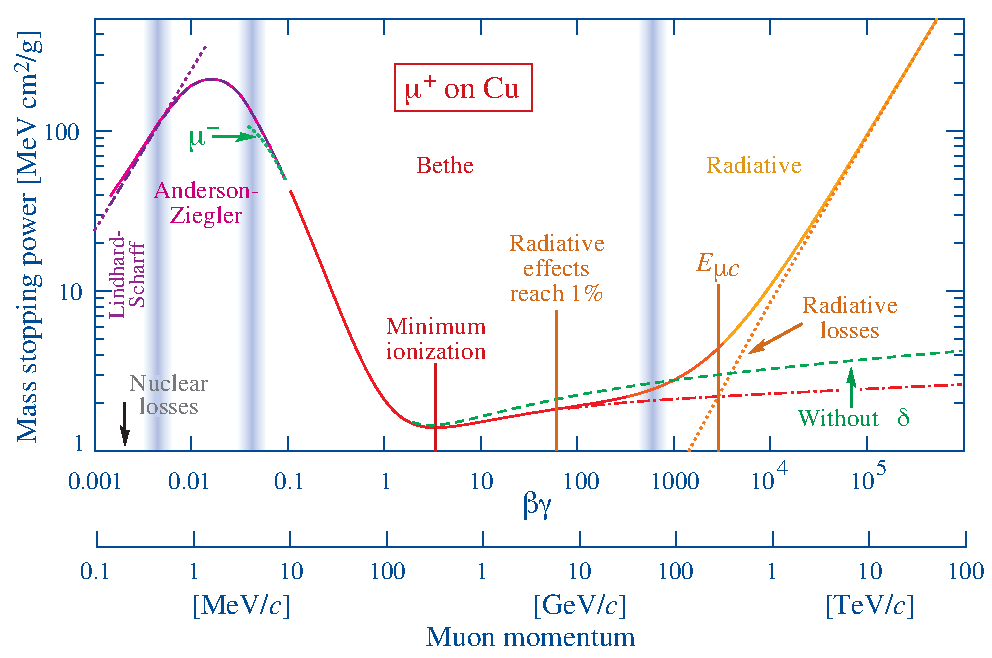
\includegraphics[width=0.7\linewidth]{chap2/fig/rpp_icru49_cu_col.pdf}
  \caption{Mean energy loss of muons in copper as a function of particle momentum. Vertical bands indicate boundaries between model transitions. Taken from \cite{Patrignani:2016xqp}.} \label{fig:BetheBloch}
\end{figure}

Below 100 GeV, ionization effects dominate in the energy loss and present a broad minimum around 1 GeV ($\beta\gamma \sim 2-4$). Particle in that region are generally referred as \textit{Minimum Ionizing Particles} (MIPs). Above 100 GeV, radiative effects become more important than ionization.

However, due to large fluctuations in energy transfer, the mean energy loss may differ from the $\left<\frac{dE}{dx}\right>$ calculation in "relatively" thin materials. The energy loss distribution can be described by a Laudau-Vavilov distribution. The most probable value (MPV) for the energy loss distribution is below the value of $\left<\frac{dE}{dx}\right>$ by around 60\% and has a long tail toward high energy losses due to:
\begin{itemize}
  \item The production of $\delta$-electrons when a significant amount of energy is transferred in a collision
  \item Bremsstrahlung photons that initiate small EM Showers
  \item Nuclear reactions of the muon with the nucleus of the material giving rise to high local energy deposits
\end{itemize}
For thick materials, the distribution becomes more Gaussian-like.

\subsection{Hadronic showers}

Charged hadrons

\section{Calorimeters}

\subsection{Energy resolution}

\subsection{Compensation}

\subsection{Sampling calorimeters}

\section{Pandora, a Particle Flow Algorithm}
\label{sec:PFA}
